\startchapter{Related Works}
\label{chapter:problem}

\newlength{\savedunitlength}
\setlength{\unitlength}{2em}

Many variants of CAs have been proposed in a vast range of different applications such as single and multi-objective optimization, dynamic problems, social interactions simulation. Here, we are interested in studying socially motivated and multi-population variants as some modern approaches in solving optimization problems.
\section{Cultural Algoithms}
\subsection{Heterogeneous Multi-Population Cultural Algorithm}
\cite{kobti2013heterogeneous} proposed a new architecture for cultural algorithms. In this pproach, the whole population is divided into a set of independent sub-populations which work in parallel without direct communication. They referred to the works of \cite{xu2010novel} \cite{guo2011novel} \cite{vasile2011inflationary} \cite{sharma2011reserve}. As their motivation they stated that most of proposed variants of evolutionary algorithms suffers from immature convergence. This occurs because these algorithms can not hold the diversity at a reasonable level. Based on existing research works, they hypothesized that multi-population streategies would be a better choice as they have the potential to perfrom an efficient search on complex landscapes. In their approach, the optimization parameters are divided among some heterogenous sub-populations. the sub-populations are called heterogenous because each sub-population is responsible for optimizing a different subset of parameters. Each sub-population represents a partial solution instead of a complete solution. To evaluate a partial solution, it gets completed by its complement parameter values from the belief space. The complete solution is evaluated based on a numerical optimization function. Also, to make the convergence process faster a simple local search strategy is incorporated into the proppsed algorithm. The general architecture of their algorithm is presented in Figure \ref{fig:HPMCA} \newline
\begin{figure}[h]
	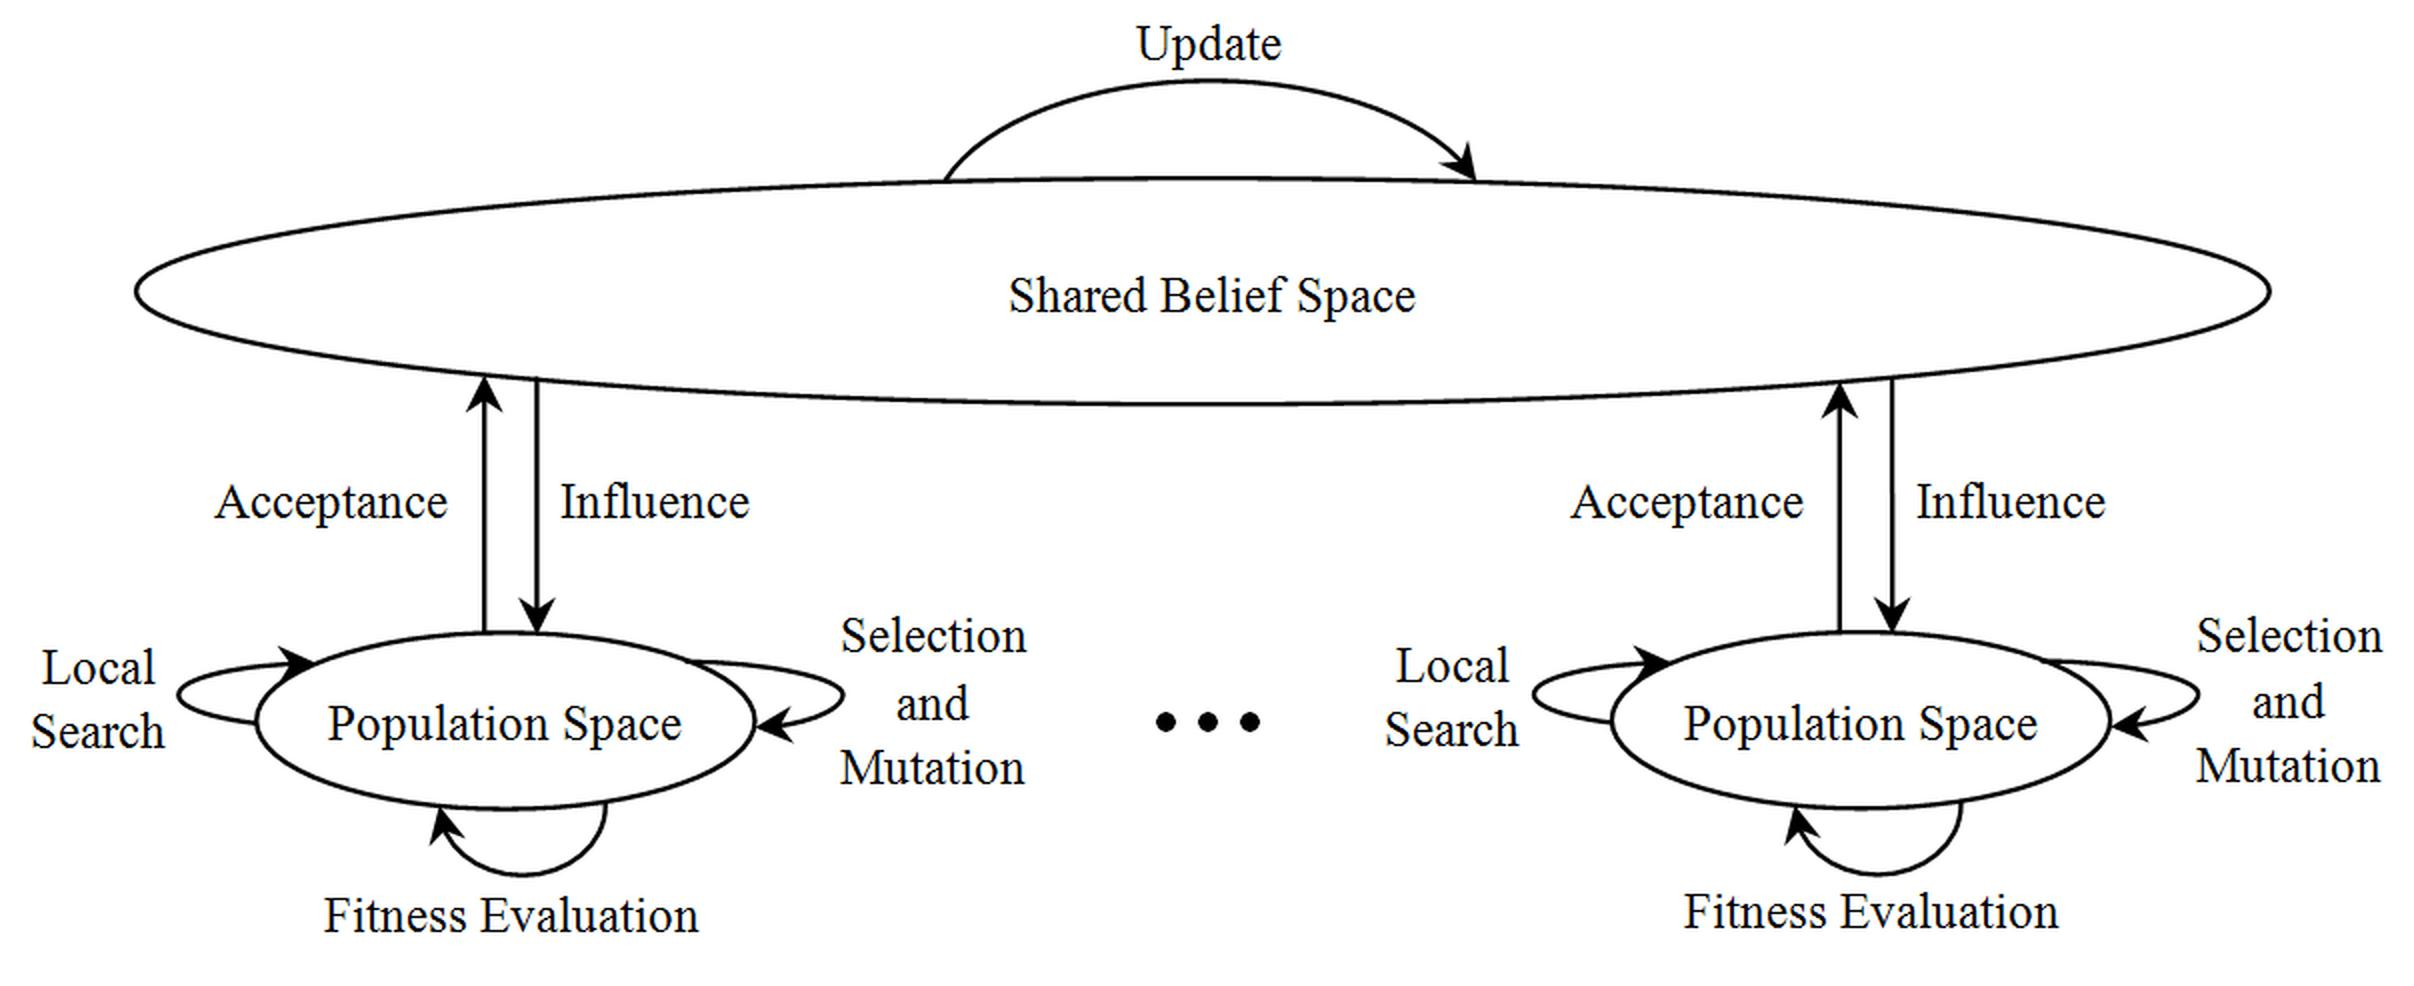
\includegraphics[scale=0.18]{HMPCA}
	\centering
	\caption{H-MPCA Architecture \cite{kobti2013heterogeneous}}
	\label{fig:HPMCA}
\end{figure}
In the experiments, they considered the whole population size to be 1000 individuals. It is divided into 30 sub-populations. So, the size of each sub-popualtion is 33. The algorithm runs for the maximum of 10000 generations and the local search strategy runs only for 10 iterations. They evaluated HMP-CA on a set of 8 complex optimization functions. It is able to find the minimum value for 7 functions out of 8. However, when the local search strategy is applied to the expriments, the proposed method outperforms all of the functions and it finds the optimum value very quickly. Ultimately, they claimed that their porpsed approach is efficient in both time and space complexity.

\subsection{The Social Fabric Approach as an Approach to Knowledge Integration in Cultural Algorithms}	
\cite{reynolds2008social} begins with a brief introduction to socially motivated methods to problem solving. They referred to the works of \cite{hu2003engineering}, \cite{reynolds2007exploring}, and \cite{cheng2005weaving}. It compares qualities of Ant Colony Optimization (ACO), Particle Swarm Optimization (PSO), and Cultural Algorithms (CA) regarding the scale in which the interactions between agents occur. Figure \ref{fig:SFAPP} compares PSO, ACO, and CA in terms of the time and space continuum over which the social interactions occur. Individuals in ACO and PSO tend to interact in a reatively limited temporal and spatial scales. It is obvious because the agents in both ant and paricle swarm algorithms exchange information with only other agents in their local neighborhood. On the other hand, cultural algorithms let the individuals interact together using various types of symbolic information emerged from complex cultural systems. In cultural algorithms the interactions among individuals occur indirectly through a shared belief space. So, cultural algorithms allow individuals interact in a global scale.
\begin{figure}[h]
	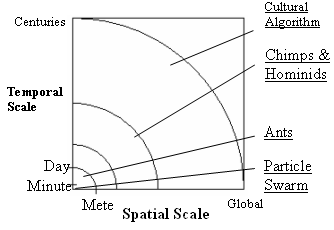
\includegraphics[scale=0.9]{SFAPP}
	\centering
	\caption{Scale of social interactions\cite{kobti2013heterogeneous}}
	\label{fig:SFAPP}
\end{figure}
Then, they asked the essential question of what social structures might emerege alongisde the search process?. To answer such questions, they introduced a new influence function which utilizes the social fabric phenomena. The old influence function assumes no interactions between agents and works based on the simple roulete wheel method. On the other hand, in the new influence function, the individuals are connected through a social network (fabric). Multiple layers of such networks could be employed in a population. The interplay of these network connection forms a social fabric. At each iteration, an individual could specify its controller knowledge source. In this approach, the contoller knowledge source is chosen based on the majority of knowledge sources in the neighborhood of an individual. The neighborhood size of an individual is specified by the topology of the fabric. Inspired by Particle Swarm Optimization literature, different topologies could be taken into consideration to model the relationships among individuals. In their work, they only considered Ring and Square topologies. They stated that, the topology of the social fabric determines the extent to which the influence of knowledge sources could be spread thorugh the network.\newline
To evaluate the social fabric approach, they implemented it in Repast frameork. Repast is a simuation tool for multi-agent systems. They created a cultual algorithms toolkit (CAT) to view the capabilities of cultural algorithms in solving various problems. They chose Cone World problem to evaluate and compare their approach with the standard cultural algorithm. The reason that they chose this problem is that by changing its parameters during the evolution process, it can show a dynamic behavior. So, Cone World problem provides an efficient way to test flexibility of search algorithms. They set the parameters of CAT as: 100 individuals, 100 cones and 1000 generations. They used ring and square topologies to from he social fabric. They stated that square topology works better than ring as it finds the solution after 250 iterations. While, the ring topology finds the best solution 450 iterations.
\subsection{Robust Evolution Optimization at the Edge of Chaos: Commercialization of Culture Algorithms}
The authors of \cite{che2010robust} aimed at commercializing Cultural Algorithm Toolkit (CAT) thourgh developing a robust variant of it. By robustness, they mean to develop a cultural algorithm which is capable of being applied across a vast range of complex problems. At first, they referred to \cite{peng2005knowledge} as an standard model cultural algorithms which assumes no connection between individuals. Then, they referred to \cite{ali2008using}, which introduced the concept of social fabric to allow individuals interact together. The authors extended the work of Ali by allowing the social networks having a memory. In addition, they utilized a variety of different networks in order to deteremine the relationship between network and problem complexity. \newline They brought up the hypothesis that there might be multiple independent networks for different purposes such as kinship and economics. In such networks, there are always some individuals which are member of multiple networks and so, they can play the role of mediator between differet networks. To preserve the diversity, the authors utilized a variety of different topologies such as Lbest, Square, Hexagon, Octagon, Hexadecagon, and Gbest. \newline
They stated that in the previous work of \cite{ali2008using}, he employed an un-weighted majority win strategy to determine the contoller knowledge source of an individual. It just relied on the count of each knowledge source in the neighborhood of each individual. The authors replaced it with a new strategy which use the average fitness of each KSs instead of each KSs count. So, the performance of individuals in a neighborhood influences which knowledge source to be chosen for the next iteration. \newline
To evaluate the robustness of the algorithm, the authors used Cone World Generator \cite{morrison1999test} as a dynamic problem. Reffered to the work by \cite{lewin1999complexity} ,they defined three classes of entropy in the connes world problem:
\begin{enumerate}
	\item Fixed: There is a low entropy and the parameters of the environment do not tend to change at all.
	\item Periodic: The environment parameters change in a regular period of time. So, the algorithm should be capable adapting itself regularly.
	\item Chaotic: In this case, the parameters change without any order and no prediction could be made about them. In fact, it is more similar to real-world cases.
\end{enumerate}
For the fixed category, the square topology successfully solved 84\% of the problems and as the best topology. For the periodic case, the octagon topology showed a better performance than other toplogies. And, for the chaotic category, Gbest showed a better result mostly in terms of average time to find a solution and the standard deviation. In summary, as the complexity of problems grows, there is the need for more connections between individuals in a social fabric to keep the robustness of the algorithm.
\subsection{Socio-Cultural Evolution via Neighborhood-Restructuring in Intricate Multi-Layered Networks}
The authors of \cite{ali2012socio} aimed at exploring the utilization of neighborhoods in the population level of cultural algorithms and see how it influences the knowledge swarming in the belief space. Their approach uses a dynamic neighborhood restructuring to preserve diversity efficiently. They referred to the reasearch works of \cite{elsayed2011differential}, \cite{asafuddoula2011adaptive}, \cite{asafuddoula2011adaptive}. Those papers proposed some adaptive methods which tried to make a trade-off between exploration and eploitation properties of evolutionary algoithms. Among the referred papers, the work by \cite{ali2010enhancing} used the social fabric phenomena to from multi-layered hierarchical network structures in both homogenous and heterogeneous networks. Figure \ref{fig:MLAYER} describes the multi-layered structure.\newline
The authors defined the social fabric phenomena as follows:
\begin{displayquote}
	"The Social Fabric is a living informational skin created out of the engineered emergence of agents illustrating the tension between the individual and the community in a context of interaction between them"
\end{displayquote}
\begin{figure}[h]
	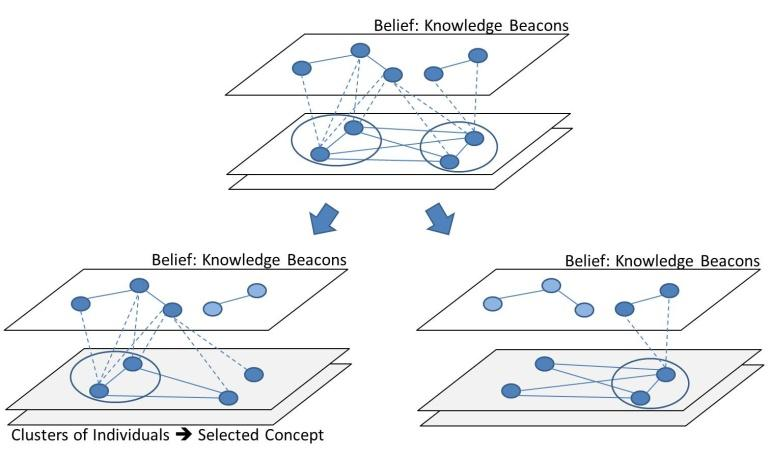
\includegraphics[scale=0.35]{MultiLayer}
	\centering
	\caption{Multi-Layered Social Network with CA \cite{kobti2013heterogeneous}}
	\label{fig:MLAYER}
\end{figure}
The informational skin is created by the connectivity of individuals together. The social fabric is used to combine the behaviors at both indivials and society levels. Then, they proposed a strategy to determine the contoller knowledge source of each individual in each generation. In the strategy, the agents send the name of their contoller knowledge source to their neighbord through the social fabric. Each individual picks the mostly used knowledge source in its neighborhood as its controller for the next iteration. In case of a tie between two or more knowledge sources, three tie-breaking strategies are intorduced:
\begin{enumerate}
	\item Most Frequently Used (MFU)
	\item Random
	\item Least Frequently Used (LFU)
\end{enumerate}
They stated that their proposed approach is inspired from a previous work of \cite{reynolds2008mining}. The new idea was called Cultual Algorithm with Restructuring Layered Social Fabric (CARLSOF). In this approach, the whole population is divided into two layers of rudimentary and advanced members. There are some independent tribes in the population space which their best performing individuals form the advanced layer and the others form the rudimantary level. In the previous works, the topology of social fabrics were supposed to be fixed and homogenous. They utilized a variety of regular topologies to form the social fabric. The authors proposed a new strategy to enable the fabric to be restructured in the case of stagnation. Each tribe may decide to change its topology to a denser (with more conections) or sparser (with less connections). They referred to two different restructuring strategies as similar approaches. The first one was Layered Delaunay Triangulation which is based on voronoi diagram. The second approach was Random Rewiring Procedure which starts with a regular topology and then rewire each edge randomly with the probability $p$. \newline
To evaluate the performance of CARLSOF, they used function set of IEEE-CEC2011 evolutiosry competition. The algorithm was implemented in JAVA. The authors reported that CARLSOF was successful to enhance all of the functions in the testbed interms of average, best, and worst obtained values. Also, they claimed that CARLSOF outperforms the best previously obtained results for European Space Agency (P12) and Casini (P13) problems results. They reported 2.983 km/sec compared to previous best 7.095. For p13, they reported 8.383091 km/sec compared to previous best 8.3832.
\subsection{Leveraged Neighborhood Restructuring in Cultural Algorithms for Solving Real-World Numerical Optimization Problems}
In the paper \cite{ali2016leveraged}, the authors made an overall review of related works on Cultural Algorithms and Social Fabric \cite{peng2005knowledge}, \cite{reynolds2008social}, \cite{chen2006tribe}, and \cite{785509}. They introduced the concept of social fabric as an infrastructure which facilitates the propagation of the influence of the knowledge sources thorugh the population space. The whole population is divided into multiple small sized tribes. Unlike other PSO-based multi-swarm variants, the tribal sub-swarms change their topology during the evolution process to keep diversity against stagnations.\newline
The tribes are organized in a two-layer structure of advanced and rudimentary classes. The advanced calss is composed of best perfoming individuals of each tribe. From each tribe, two examplars are chosen. The first one is the best of explorer knowledge sources (Normative and Topopgraphic) and the second one is the best of exploiter knowlegde sources (Situational). Figure \ref{fig:TwoLayerSF} describes the two-layer structure. The authors utilized only three kinds of knowledge sources: Normative, Topographic, and Situational. They claimed that, other types of knowledge sources are suitable for dynamic problems. However, they used a set of static problems to evaluate their approach. The authors divided the evolution process of CAs into three stages: the secluion stage , the rapport stage , and the cohesive stage. In the seclusion stage, the tribes evolve independetly and without any exchange of information. Then, in the rapport stage, the tribes start to exchange knowledge via the advenced class. Also, the neighborhood restructuring strategy is lunched in each tribe. So, the tribes have the capability to restructure their topology to keep diversity and avoid local optima. The first two stages ensure that diversity has been kept in the initial iterations of the search process. Finally, in the third stage, all the tribes are merged together and continue the search process as a single CA model.
\begin{figure}[h]
	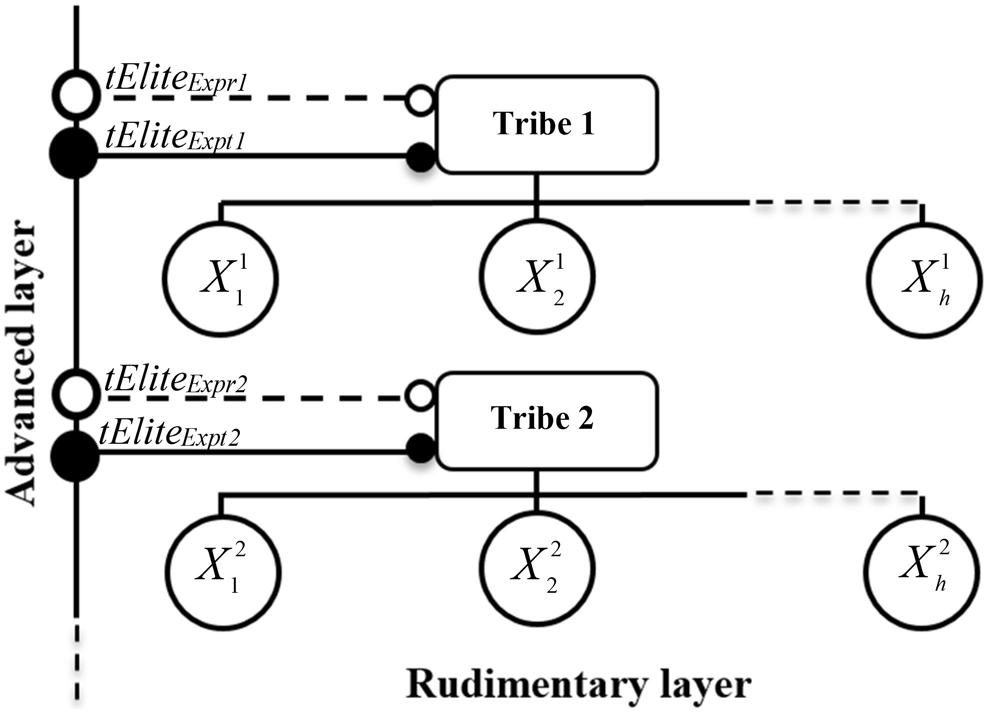
\includegraphics[scale=0.25]{TwoLayerSF}
	\centering
	\caption{Two-class taxonomy of the tribal CA \cite{kobti2013heterogeneous}}
	\label{fig:TwoLayerSF}
\end{figure}
Based on the categorization proposed in \cite{de2009heterogeneous}, the authors claimed that their apparoach is heterpgeneous regarding update-rule heterogeneity and neighborhood heteogeneity. Since the topology of each tribe is changing during the evolution process, the tribes might use different toplogies at the same time. So, it could be considered as heterogenous neuighborhood restructuring. Also, their approach utilizes update-rule heteogeneity because, there are individuals with different roles (explorer and exploiter). \newline
In the exprimental results section, the authors used IEEE-CEC2011 competition on testing evolutionary algorithms on real-world numerical optimization problems. They presented an extended comparison of their approach with other propsed methods. At first, the authors tested the approach (T-SCANeR) with different values for these parameters: tie-breaking rule, $M_{thresh}$, and number of elites. There is no best value for tie-breaking rule as it is problem-dependent. For the $M_{thresh}$ parameter, the results show that the best value is 50. The best value for $n_{tElite}$ is 2. The second expriment was on varying the  window  size  within  which  the  social  fabricis  applied  and  aggregated ($W_{size}$). The best reported value for $W_{size}$ is 20. \newline
In the two first exprients the best values for the parameters were determined. Based on the obtained values, the authors compared T-SCANeR with five other evolutionary algorithms on the IEEE-CEC2011 which is a set of 18 functions. T-SCANeR managed to outperform for most of the functions except for $T_{3}$, $T_{4}$, $T_{6}$, and $T_{11.5}$. Problems $T_{12}$ (full messenger problem) and $T_{13}$ (cassini problem) are associated with the European Space Agency (ESA). The authors claimed that T-SCANeR outperformed other methods by 2.193724 km/s for the messenger problem and 8.383090 for the cassini problem.
\section{Particle Swar Optimization}
\subsection{Tribe-PSO: A novel global optimization algorithm and its application in molecular docking}
The authors of \cite{chen2006tribe} proposed a new variant of Particle Swarm Optimization (PSO) called Tribe-PSO for the primary purpose of molecular docking in chemometrics. As some previous research work, they referred to \cite{jones1997development} and \cite{clerc2002particle}. Their approach is inspired from Hierarchical Fair Competition concept \cite{jianjun2002adaptive}. They divided the whole population into some tribes and the evolution process into three phases. The tribes are organized into two layers of basic and upper individuals. \newline The individuals in each tribe are completely isolated from other tribes. So, they form the basic layer. On the other hand, the best members of each tribe can see the other tribes and exchange information with their best members as well. The problem-solving process is divided into three phases: isolated, communing, and united. In the first phase, the tribes are completely isolated and there is no exchange of information. In the second phase, the two-layered model is formed and the tribes begin to exchange information through their best performing individuals. In the third phase, all the tribes are merged into a single popualtion. Then, it operates as basic PSO model until meeting some stopping criteria. The autohrs claimed that their approach helps the individuals preserving diversity and avoiding local optima against multi-modal solution spaces.\newline
The authors used two testbeds to evaluate and compare the performance of Tribe-PSO with standard PSO. The first was De Jong's function set and the second was a test set of 100 receptor-ligand X-ray structures selected for docking benchmark. In the De Jong's testbed, the basic PSO showed a better performance in the isolated phase. However, in the communing phase Tribe-PSO converged to a better value than basic PSO. In the unity phase, the basic PSO seemed to get stuck in a local optimum. However, Tribe-PSO continued to accelerate convergence and got better results than basic PSO. In the docking benchmark, Tribe-PSO was compared to the AutoDock library. Four parameters are calculated after 10 independent runs: Best, Run1, Average, and Standard Deviation of the results. The relative difference of the four benchmark factors between Tribe-PSO and AutoDock were calculated. The results for the four factors showed that Tribe-PSO leads to a better performance than AutoDock.
\subsection{Heterogeneous Particle Swarm Optimizers}
The authors of \cite{de2009heterogeneous} peresented a survey on heterogeneous variants of Paritcle Swarm Optimization (PSO). They claim that the homogenous models have been attractive because of their simplicity in conceptual and application levels. However, heterogeneous models are ubiquitous in nature. Here, heterogeneity means the individuals may differ from each other regarding their parameters and search behavior. \newline 
At first, the authors presented a breif description of three well-known variants of PSO: Accelerated PSO \cite{zhang2003adaptive}, Fully-informed PSO \cite{mendes2004fully}, and Bare Bones PSO \cite{kennedy2003bare}. Then, they authors categirzed the heterogeneous variants of PSO into four categories:
\begin{enumerate}
	\item Neighborhood
	\item Model of Influence
	\item Update Rule
	\item Parameters
\end{enumerate}
Neighborhood heterogeneity refers to the cases that the topology of the swarm is not regular. This type of heterogeneity occurs when the neighborhood size of each individual is different. They claimed that the neighborhood heterogeneity allows some population to be more influential than otehrs. Individuals with higher number of connections have the potential to attract more individuals through the search process. [Kennedy ref]\newline
Model of Influence heterogeneity refers to the situations that the individuals employ different strategies to specify their informers. The word Informer refers to an individual which is going to influence another individual. []\newline
Update-rule heterogeneity means the individuals utilize different strategies to update their position in the search space. This kind of heteogeneity makes it possible for the individuals to explore the search space in several ways. Also, the particles can play different but complementary roles. For example, some of them may tend to explore unseen parts of the solution space and some others only follow those scout individuals. The second type are the exploiters.\newline
Parameter heterogeneity occurs when some individuals in a group which follow the same update rule use different update rule's parameter settings. Having different search parameters, even in a group of similar particles, leads to various search behaviors which improves the level diversity. The authors referred to [], [] ,[] which utilize different initial values for the parameters such as acceleration coefficient, maximum velocities and inertia weight.\newline
To compare the mentioned categories, the authors careted two test cases. The first one compared two PSO variants with different update rules: Velocity-based and Bare bones swarm. The evaluation results confirmed that velocity-based outperformed the other one. The second test case compared two PSO variants with different models of influence: best-of-neighborhood and fully-informed swarm. The evaluation results showed that the fully-informed algorithm outperfromed the best-of-neighborhood.

\section{Chapter Conclusion}
From the chosen research works, we will be utilizing the concept of heterogeneous neighborhood structures by \cite{de2009heterogeneous} to improve the robustness of social fabric-based cultural algorithm \cite{ali2016leveraged}. We replace the population component of \cite{ali2016leveraged} with PSO algorithm.


